% mainfile: ../../piOZ.tex
As mentioned previously, the word \textit{mobile} refers to the information sharing and evolution, since the receiver process may use the received information to change its location. For example, consider the process: $\procres{x,y}{(\procpar{\proccall{A}{x,y}}{\proccall{B}{x}})}$ where:
\begin{itemize}
\item $\procdef{A}{a,b}\define{}\out{a}{{b}}.\proccall{A}{a,b}$
\item $\procdef{B}{c}\define{}\inp{c}{{d}}.\proccall{B}{d}$
\end{itemize}


\refLis{pi_mobility_stargazer_code} shows its the stargazer code,  \refFig{pi_mobility_stargazer_react} shows its visualization before and after the interaction occurrence.
\lstinputlisting[backgroundcolor=\color{white},caption={Stargazer code for the process $\procres{x,y}{(\procpar{\proccall{A}{x,y}}{\proccall{B}{x}})}$.},captionpos=b, label={pi_mobility_stargazer_code}]{listings/pi_mobility_stargazer_code.pi}
\raggedbottom

\begin{figure}[H]%
\centering
\subcaptionbox{Before reaction occurrence.}{\fbox{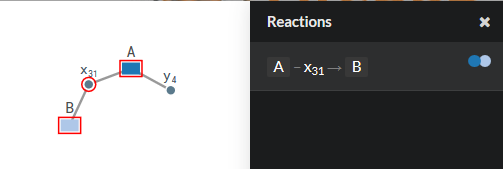
\includegraphics[width=0.45\textwidth]{./images/pi_mobility_stargazer_Before_react.png}}}%
\hfill
\subcaptionbox{After reaction occurrence.}{\fbox{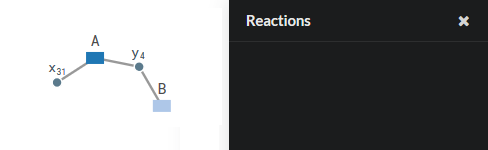
\includegraphics[width=0.45\textwidth]{./images/pi_mobility_stargazer_After_react.png}}}%
\caption{Mobility reaction}
\label{pi_mobility_stargazer_react}%
\end{figure}


Intuitively, The mobility can be noticed in \refFig{pi_mobility_stargazer_react}, since $B$ changed it's position in the connection topology.
The following explains the mobility through interaction step by step:
\begin{itemize}
\item Initially the process $\proccall{A}{x,y}$ has the channels $x,y$ and the process $\proccall{B}{x}$ has the channel $x$. Thus, $\proccall{A}{x,y}$ and $\proccall{B}{x}$ are connected via channel $x$.
\item $\proccall{A}{x,y}$ has commitment $\out{x}{{y}}$, i.e., send the channel name $y$ via the channel $x$.
\item $\proccall{B}{x}$ has commitment $\inp{x}{{d}}$, i.e., receive a message $d$ via $x$.
\item That means: a reaction can occur between $\proccall{A}{x,y}$ and $\proccall{B}{x}$. This reaction is: $\procres{x,y}{(\procpar{\out{x}{{y}}.\proccall{A}{x,y}}{\inp{x}{{d}}.\proccall{B}{d}})} \transs{\tau} \procres{x,y}{(\procpar{\proccall{A}{x,y}}{\proccall{B}{y}})}$.
\item Information sharing: the process $\proccall{A}{x,y}$ sends the name $y$ to $\proccall{B}{x}$ when the interaction occurs.
\item Evolution: when interaction occurs $\proccall{B}{x}$ knows about the channel $y$ and uses it as parameter for the the process call $\proccall{B}{y}$ .i.e, The  $\proccall{B}{y}$ now has the channel $y$, and no more $x$.
\item Finally, in other words: 
\begin{itemize}
\item before the reaction: $B$ was connected to $A$ via $x$ as shown in \refFig{pi_mobility_stargazer_react}.
\item after the reaction: $B$ is connected to $A$ via $y$ as shown in \refFig{pi_mobility_stargazer_react}.
\end{itemize}
\end{itemize}
